\subsection{Molecular Dynamics}
\begin{frame}{Dynamics Simulation}
The standard steps of a dynamics simulation are as follows:
\vspace{1cm}
\begin{enumerate}
	\item Minimisation 
	\begin{itemize}
		\item 0 K 
	\end{itemize}
	\item Heat
	\begin{itemize}
		\item 0 K to 300 K, Constant volume
	\end{itemize}
	\item Equilibration
	\begin{itemize}
		\item 300 K, Constant volume and pressure
	\end{itemize}
	\item Production dynamics
	\begin{itemize}
		\item 300 K, Constant volume and pressure
	\end{itemize}
\end{enumerate}
\end{frame}

\begin{frame}{Setup}
Molecular dynamics simulations require an initial parameter and structure file to run.
\vspace{1cm}
\newline
We need to:
\begin{enumerate}
\item Create separate files for the Mg\textsuperscript{2+} and Diphosphate ions
\item Load parameters for the protein, ligands and solvent
\item Join these files, plus the docked ligand
\item Solvate the system
\item Neutralise the system
\item Generate parameters and coordinate files
\end{enumerate}
\end{frame}

\begin{frame}{Box shape}
\begin{columns}
\column{0.5\textwidth}
\begin{itemize}
	\item Solvent molecules dominate simulation time
	\item Reducing the amount of solvent speeds up simulations
	\item Want the periodic box to be optimised to reduce solvent molecules
	\item Truncated octahedron is generally a good shape for \enquote{round} proteins
\end{itemize}
\column{0.6\textwidth}
\begin{figure}
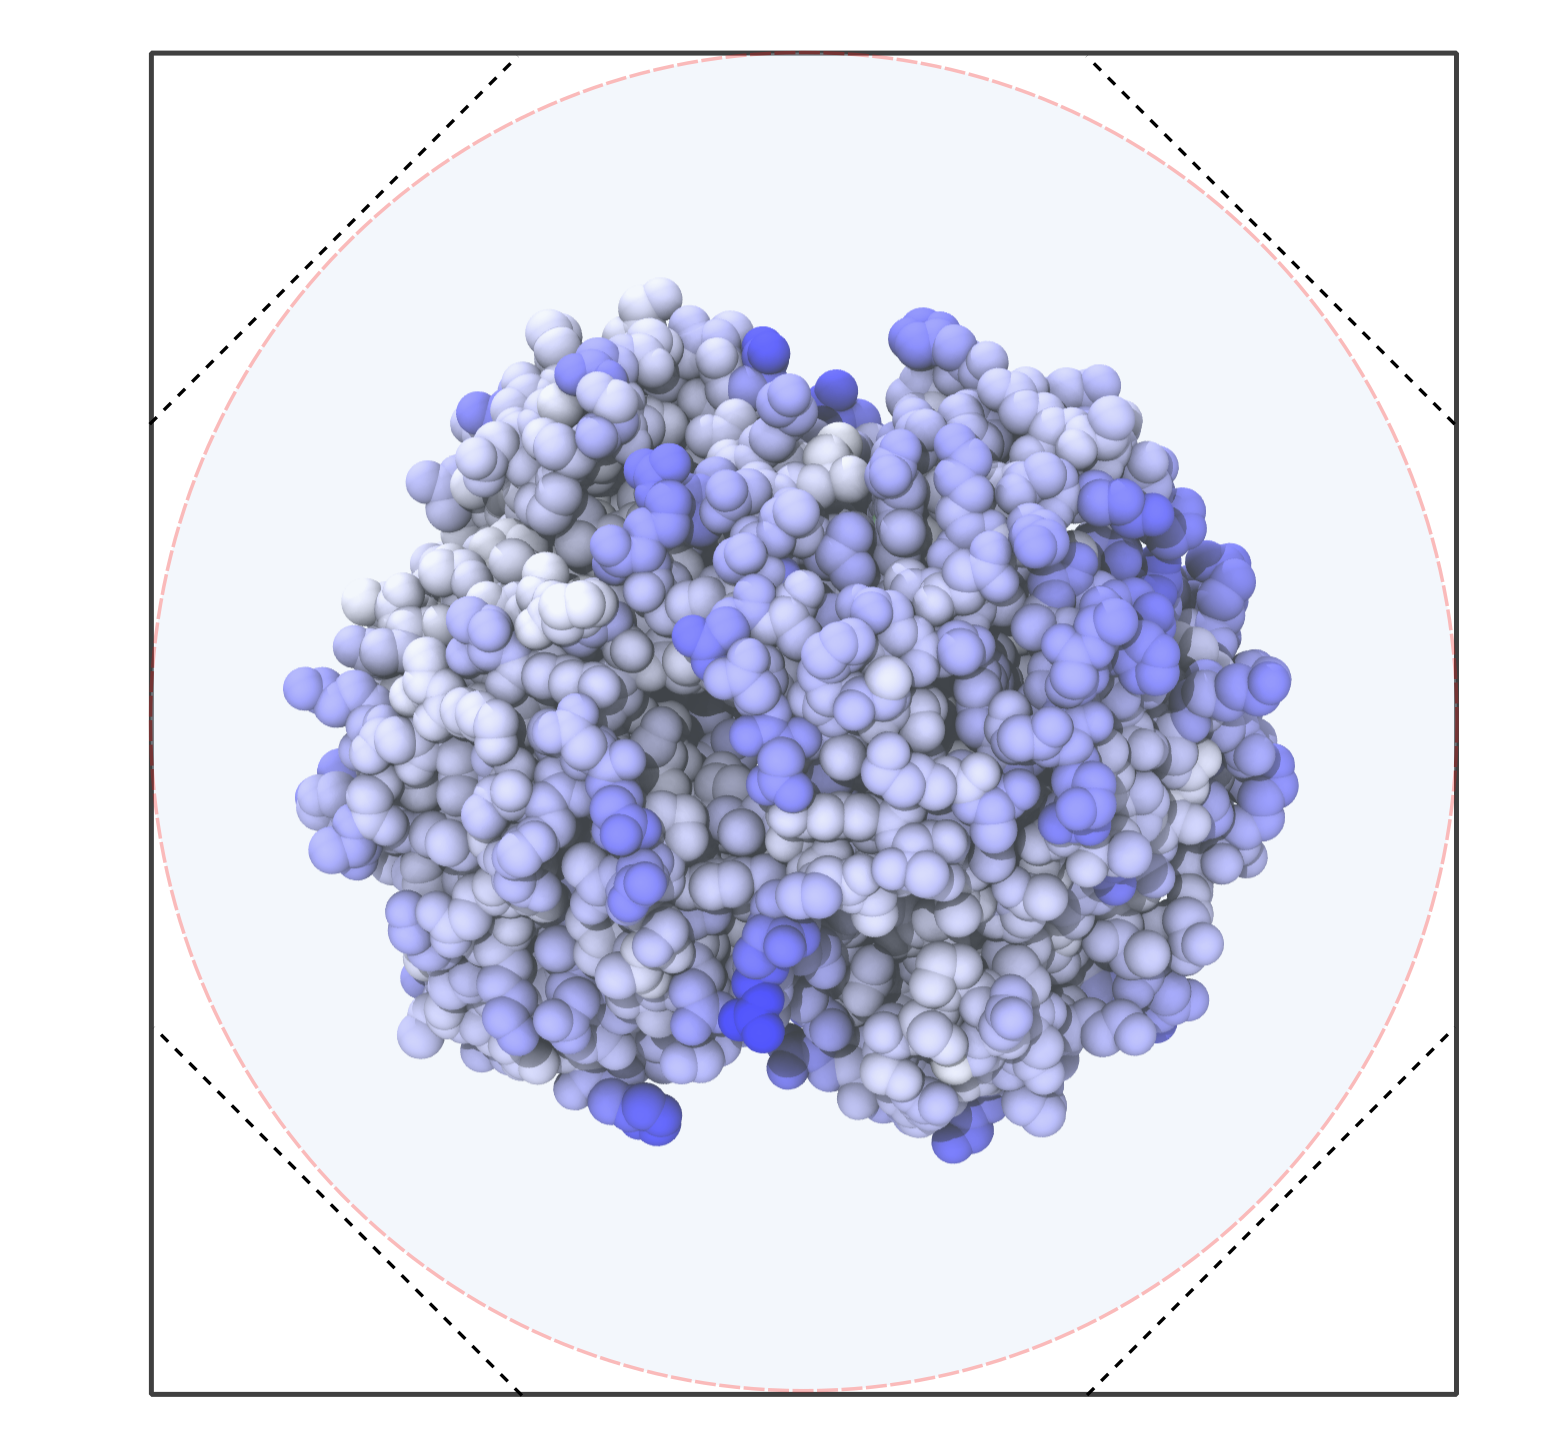
\includegraphics[height=0.7\textwidth]{figures/theory/cubic_box.png}
\end{figure}
\end{columns}
{\tiny Figure: \href{https://computecanada.github.io/molmodsim-md-theory-lesson-novice/04-Periodic_Boundary/index.html}{https://computecanada.github.io/molmodsim-md-theory-lesson-novice/04-Periodic\textunderscore Boundary/index.html}}
\end{frame}
\begin{frame}{Box shape}
\begin{columns}
\column{0.5\textwidth}
\begin{itemize}
	\item Solvent molecules dominate simulation time
	\item Reducing the amount of solvent speeds up simulations
	\item Want the periodic box to be optimised to reduce solvent molecules
	\item Truncated octahedron is generally a good shape for \enquote{round} proteins
\end{itemize}
\column{0.6\textwidth}
\begin{figure}
\includegraphics[height=0.7\textwidth]{figures/theory/TruncatedOctahedron.png}
\end{figure}
\end{columns}

\end{frame}

\begin{frame}{Generate input files}
\begin{figure}
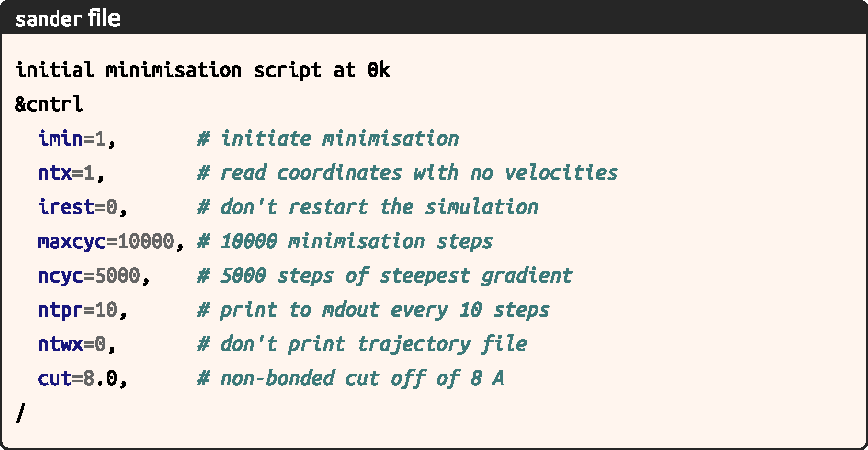
\includegraphics[height=0.7\textheight]{figures/dynamics/min.pdf}
\end{figure}
\end{frame}

\begin{frame}{Generate input files}
\begin{figure}
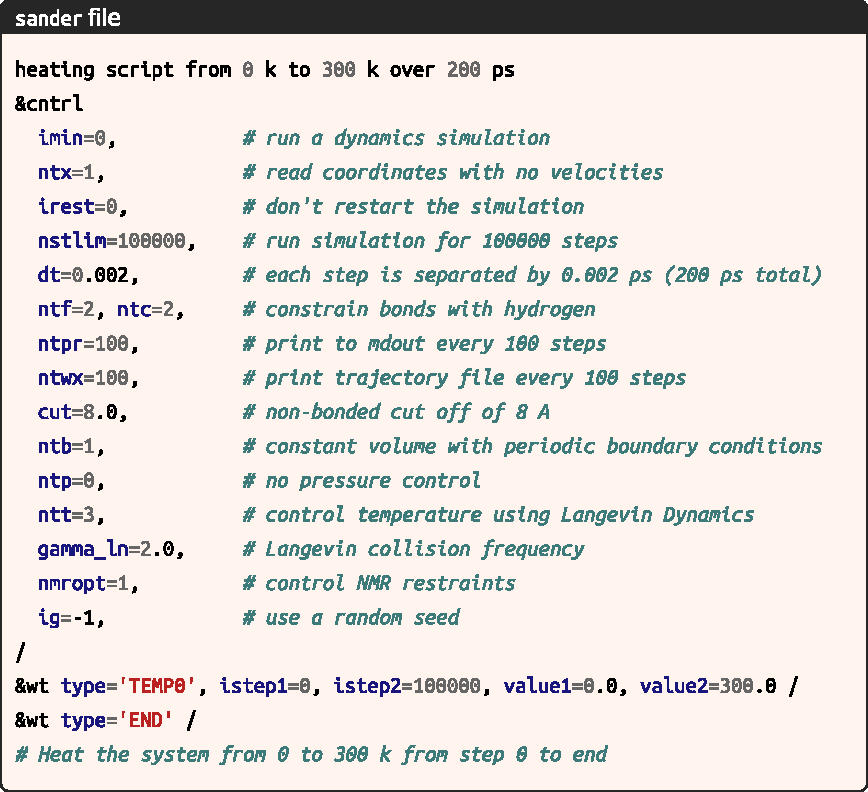
\includegraphics[height=0.8\textheight]{figures/dynamics/heat.pdf}
\end{figure}
\end{frame}

\begin{frame}{Generate input files}
\begin{figure}
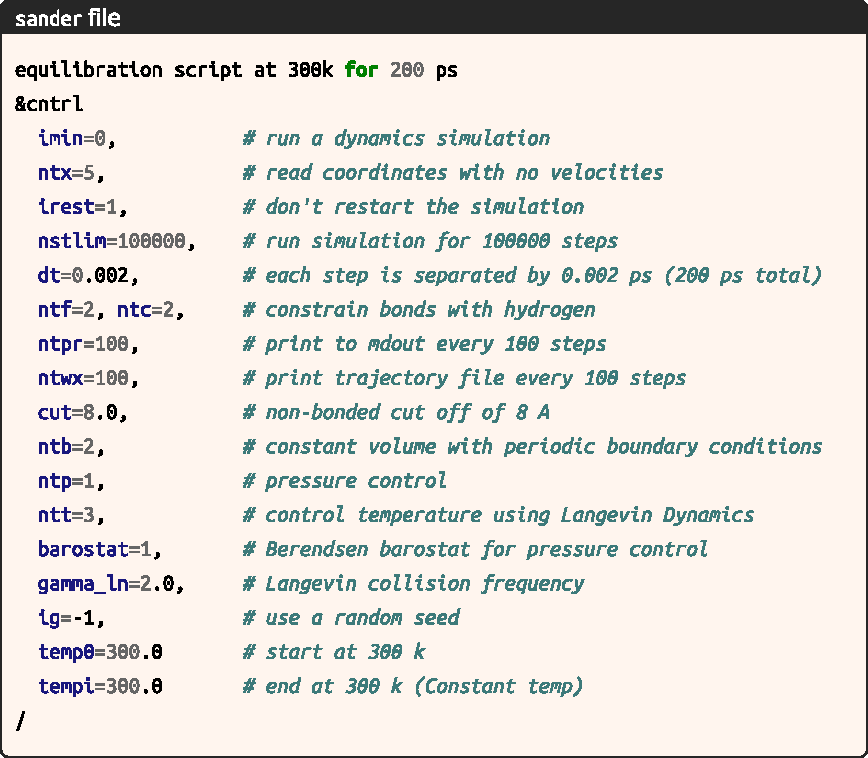
\includegraphics[height=0.8\textheight]{figures/dynamics/equil.pdf}
\end{figure}
\end{frame}

\begin{frame}{Run Simulations}
\begin{figure}
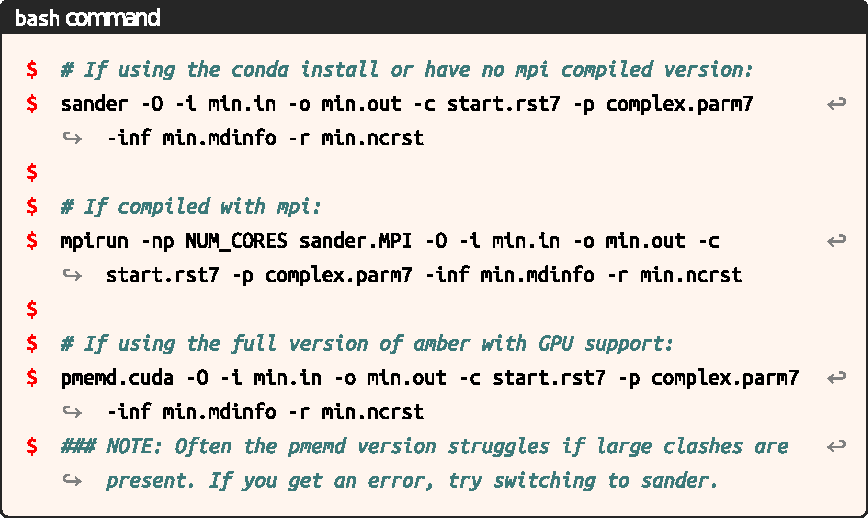
\includegraphics[height=0.7\textheight]{figures/dynamics/run.pdf}
\end{figure}
\end{frame}